\section{TODO}
\begin{itemize}
    \item SETUP: RPi setup (ubiquity)
    \item SETUP: Arduino Setup
    \item SETUP: ROS (lidar, joystick)
    \item SIMULATION: joy teleop
    \item SIMULATION: mapping
    \item SIMULATION: SLAM (hector, gmapping)
    
\end{itemize}

\section{Joystick support}
\label{section:install_joystick}
\noindent A PS3 joystick is connected via Bluetooth. Start by installing the required \texttt{joy} package:
\begin{mdframed}[backgroundcolor=light-gray, linecolor=light-gray]
\begin{verbatim}
$ sudo apt-get install ros-melodic-joy
\end{verbatim}
\end{mdframed}

\noindent Test the joystick is working by using
\begin{mdframed}[backgroundcolor=light-gray, linecolor=light-gray]
\begin{verbatim}
$ sudo jstest /dev/input/js0
\end{verbatim}
\end{mdframed}

\noindent Note that some systems may allocate a different number to the joystick other than 0. Device name can be found by using:
\begin{mdframed}[backgroundcolor=light-gray, linecolor=light-gray]
\begin{verbatim}
$ ls /dev/input/
\end{verbatim}
\end{mdframed}

\noindent Set the required permissions for ROS to access the joystick node:
\begin{mdframed}[backgroundcolor=light-gray, linecolor=light-gray]
\begin{verbatim}
$ sudo chmod a+rw /dev/input/js0
\end{verbatim}
\end{mdframed}

\noindent Test if the joystick node functions properly by running:
\begin{mdframed}[backgroundcolor=light-gray, linecolor=light-gray]
\begin{verbatim}
$ rosrun joy joy_node
\end{verbatim}
\end{mdframed}

\noindent and in  a different terminal
\begin{mdframed}[backgroundcolor=light-gray, linecolor=light-gray]
\begin{verbatim}
$ rostopic echo joy
\end{verbatim}
\end{mdframed}

\noindent In this terminal pressing joystick buttons should change the displayed values.

The next step is to create a package that would get the output from the joystick node and transform it into \texttt{geometry\_msgs/Twist} messages that would allow the movement of the robot:
\begin{mdframed}[backgroundcolor=light-gray, linecolor=light-gray]
\begin{verbatim}
$ cd ~/catkin_ws/src
$ catkin_create_pkg joy_teleop roscpp joy
$ cd .. && catkin_make
\end{verbatim}
\end{mdframed}

\noindent Next create \texttt{joy\_teleop/src/robot\_teleop\_joy.cpp } with the following contents:

\begin{listing}[H]
    \caption{This is below the code}
    \inputminted[breaklines, linenos,frame=single]{cpp}{ROS/src/robotTeleopJoy.cpp}
    \label{lst:the-code}
\end{listing}

\noindent At the end of \texttt{joy\_teleop/src/CMakeLists.txt } add the following lines:
\begin{minted}[breaklines, linenos,frame=single]{cmake}
add_executable(robot_teleop_joy src/robot_teleop_joy.cpp)
target_link_libraries(robot_teleop_joy ${catkin_LIBRARIES})
\end{minted}

\noindent Last step is to write a launch file to start all the required nodes.\\ 
Starting in the \texttt{joy\_teleop/} directory create a \texttt{launch} folder and and create the launch file \\
\texttt{joy\_teleop/launch/joystick.launch} containing the following:

\begin{minted}[breaklines, linenos,frame=single]{xml}
<launch>
 <!-- joy node -->
  <node respawn="true" pkg="joy"
        type="joy_node" name="turtle_joy" >
    <param name="dev" type="string" value="/dev/input/js0" />
    <param name="deadzone" value="0.12" />
  </node>

 <!-- Axes -->
  <param name="axis_linear" value="1" type="int"/>
  <param name="axis_angular" value="0" type="int"/>
  <param name="scale_linear" value="2" type="double"/>
  <param name="scale_angular" value="2" type="double"/>
  <remap from="robot1/cmd_vel" to="/cmd_vel"/> 
  
  <node pkg="joy_teleop" type="robot_teleop_joy" name="teleop"/>
</launch>
\end{minted}

\noindent Where at line 14 the default topic of the \texttt{joy\_teleop} node is changed to \texttt{/cmd\_vel} which is used in the next section.

\noindent The package must be built again for the changes to take effect:

\begin{mdframed}[backgroundcolor=light-gray, linecolor=light-gray]
\begin{verbatim}
$ cd ~/catkin_ws && catkin_make
\end{verbatim}
\end{mdframed}

\noindent To verify the node works as expected:
\begin{mdframed}[backgroundcolor=light-gray, linecolor=light-gray]
\begin{verbatim}
$ roslaunch joy_teleop joystick.launch
\end{verbatim}
\end{mdframed}

\noindent and in a new terminal
\begin{mdframed}[backgroundcolor=light-gray, linecolor=light-gray]
\begin{verbatim}
$ rostopic echo cmd_vel
\end{verbatim}
\end{mdframed}

\noindent At this screen by e.g. moving the left analog stick of the joystick an output of the following form can be seen:
\begin{verbatim}
---
linear: 
  x: 0.00845917593688
  y: 0.0
  z: 0.0
angular: 
  x: 0.0
  y: 0.0
  z: -0.0
---

\end{verbatim}

In this case the left analog stick was moved straigth and the \texttt{joy_teleop} node created \texttt{Twist} message that commands the robot perform alinear movement along the $x$ axis, which shows that the node is working correctly.

\section{Simulation environment}
\noindent For simulating the robot this project uses the available packages from turtlebot3\cite{web_turtlebot3_simulation}.

\begin{mdframed}[backgroundcolor=light-gray, linecolor=light-gray]
\begin{verbatim}
$ cd ~/catkin_ws/src/
$ git clone https://github.com/ROBOTIS-GIT/turtlebot3_simulations.git
$ cd ~/catkin_ws && catkin_make

echo "export TURTLEBOT3_MODEL=burger" >> ~/.bashrc
source ~/.bashrc
\end{verbatim}
\end{mdframed}

\noindent It is now possible to launch the simulation environment by running:
\begin{mdframed}[backgroundcolor=light-gray, linecolor=light-gray]
\begin{verbatim}
roslaunch turtlebot3_fake turtlebot3_fake.launch
\end{verbatim}
\end{mdframed}

\noindent and in a new terminal launch the \texttt{joy\_teleop} node:

\begin{mdframed}[backgroundcolor=light-gray, linecolor=light-gray]
\begin{verbatim}
$ roslaunch joy_teleop joystick.launch
\end{verbatim}
\end{mdframed}

\noindent This will result in launching a new \texttt{RViz} window displaying the simulated robot which moves as commanded by the joystick as can be seen in Figure \ref{figure:rviz_simulation}

\begin{figure}[H]
\centering
 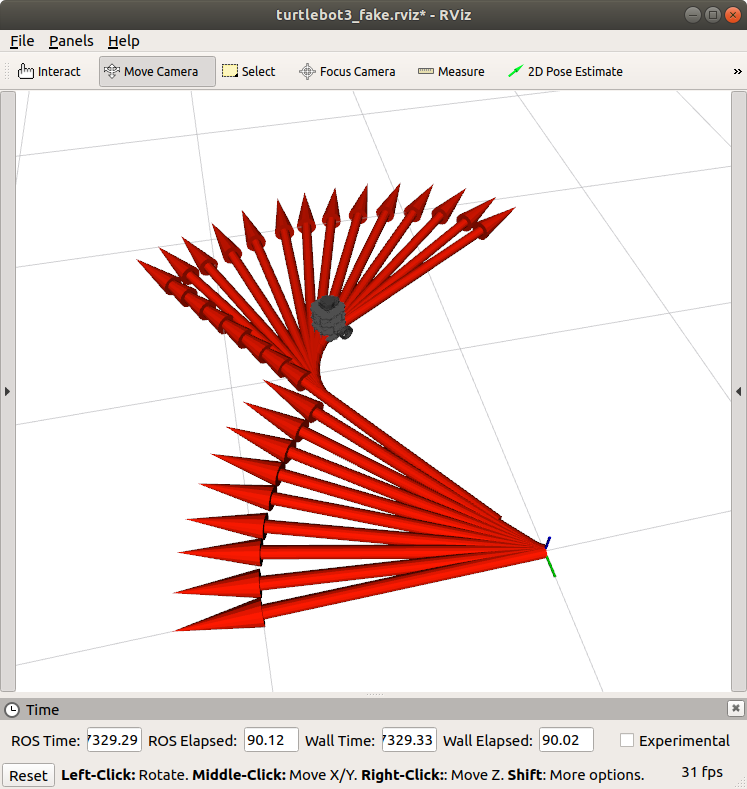
\includegraphics[scale=0.5]{Figures/ros_install/rviz_simulation.png}
 \caption{RViz windows showing the simulated robot and its commanded movement}
 \label{figure:rviz_simulation}
\end{figure}